\part{Definição da Ferramenta de Gestão}
\chapter[Definição da Ferramenta de Gestão]{Definição da Ferramenta de Gestão}

O gerenciamento de projetos é um conjunto de ferramentas destinado ao controle de eventos que estão dentro de um cenário de tempo, custo e qualidade pré determinados[1], sendo assim a definição dessas ferramentas para a gestão de um projeto é um etapa essencial na fase de Definição e Planejamento de um projeto.  

Para o projeto em questão, duas ferramentas foram selecionadas, cada uma com uma finalidade diferente, sendo elas o Trello e o Google Drive. Essas duas ferramentas foram escolhidas por disponibilizarem espaços de colaboração de grupo disponíveis online de forma livre e gratuita [2]. 

O Trello (\ref{fig:trello}) , no projeto, tem a finalidade de fazer com que todos os membros do projeto possam monitorar e acompanhar todas as etapas e atividades do projeto como um todo e fazer com o gerente do projeto consiga ter registro e controle de todas as atividades já executadas, em execução e a serem executadas.

\begin{figure}[!h]
	\centering
	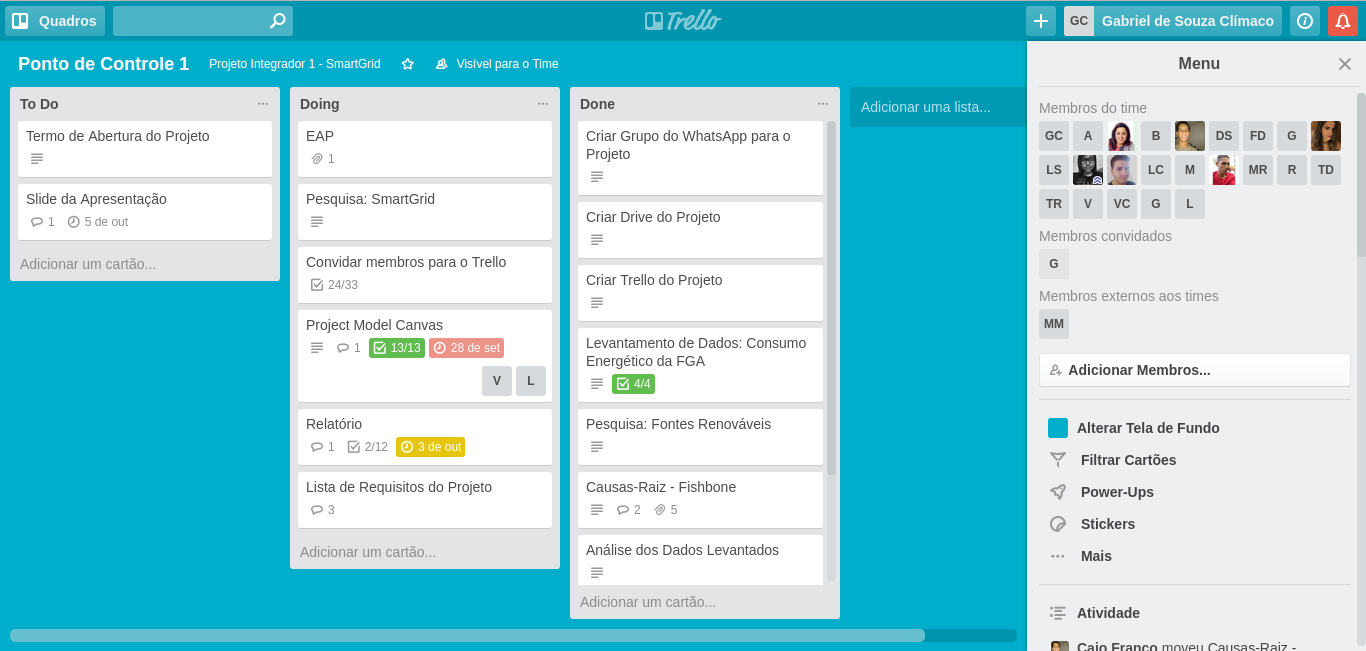
\includegraphics[scale=.7]{figuras/trello.png}
	\caption{Interface do Quadro referente ao Ponto de Controle 1 no Trello}
	\label{fig:trello}
\end{figure}

E o Google Drive (figura 2) tem a finalidade de fazer com que todos os membros do projeto possam armazenar arquivos importantes de forma compartilhada em um só lugar e permitir que eles tenham acesso ao conteúdo completo desses arquivos de forma online a qualquer momento.

\begin{figure}[!h]
	\centering
	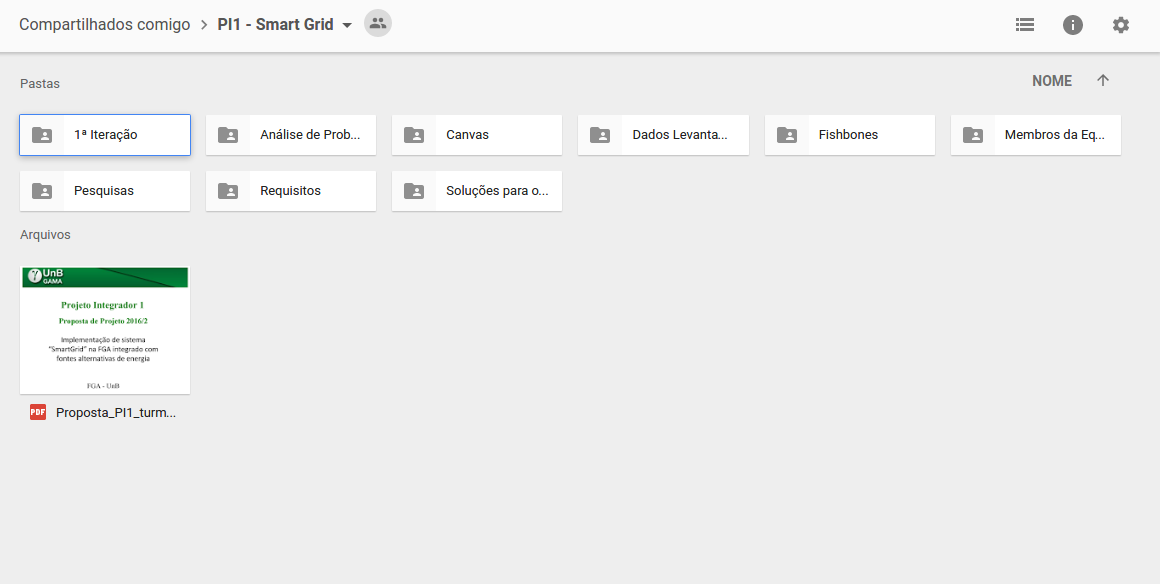
\includegraphics[scale=.7]{figuras/drive.png}
	\caption{Interface da Pasta do Projeto no Google Drive}
	\label{fig:drive}
\end{figure}

As duas ferramentas utilizadas de forma conjunta permitirá aos membros do projeto o alinhamento em relação a todas as etapas e informações do projeto. 

